\documentclass[12pt,article]{article}
\usepackage[T1]{fontenc}
\usepackage{lmodern}
\usepackage{amssymb,amsmath}
\usepackage{ifxetex,ifluatex}
\usepackage{fixltx2e} % provides \textsubscript
% use upquote if available, for straight quotes in verbatim environments
\IfFileExists{upquote.sty}{\usepackage{upquote}}{}
\ifnum 0\ifxetex 1\fi\ifluatex 1\fi=0 % if pdftex
  \usepackage[utf8]{inputenc}
\else % if luatex or xelatex
  \ifxetex
    \usepackage{mathspec}
    \usepackage{xltxtra,xunicode}
  \else
    \usepackage{fontspec}
  \fi
  \defaultfontfeatures{Mapping=tex-text,Scale=MatchLowercase}
  \newcommand{\euro}{€}
\fi
% use microtype if available
\IfFileExists{microtype.sty}{\usepackage{microtype}}{}
\usepackage[margin=1.25in]{geometry}
\usepackage{graphicx}
% Redefine \includegraphics so that, unless explicit options are
% given, the image width will not exceed the width of the page.
% Images get their normal width if they fit onto the page, but
% are scaled down if they would overflow the margins.
\makeatletter
\def\ScaleIfNeeded{%
  \ifdim\Gin@nat@width>\linewidth
    \linewidth
  \else
    \Gin@nat@width
  \fi
}
\makeatother
\let\Oldincludegraphics\includegraphics
{%
 \catcode`\@=11\relax%
 \gdef\includegraphics{\@ifnextchar[{\Oldincludegraphics}{\Oldincludegraphics[width=\ScaleIfNeeded]}}%
}%
\ifxetex
  \usepackage[setpagesize=false, % page size defined by xetex
              unicode=false, % unicode breaks when used with xetex
              xetex]{hyperref}
\else
  \usepackage[unicode=true]{hyperref}
\fi
\hypersetup{breaklinks=true,
            bookmarks=true,
            pdfauthor={Justin Murphy},
            pdftitle={Racial Bias in Stand Your Ground Cases in Florida, 2006-2013},
            colorlinks=true,
            citecolor=MidnightBlue,
            urlcolor=RoyalBlue,
            linkcolor=MidnightBlue,
            pdfborder={0 0 0}}
\urlstyle{same}  % don't use monospace font for urls
\setlength{\parindent}{0pt}
\setlength{\parskip}{6pt plus 2pt minus 1pt}
\setlength{\emergencystretch}{3em}  % prevent overfull lines
\setcounter{secnumdepth}{0}

%%% Change title format to be more compact
\usepackage{titling}
\setlength{\droptitle}{-2em}
  \title{Racial Bias in ``Stand Your Ground'' Cases in Florida, 2006-2013}
  \pretitle{\vspace{\droptitle}\centering\huge}
  \posttitle{\par}
  \author{Justin Murphy}
  \preauthor{\centering\large\emph}
  \postauthor{\par}
  \predate{\centering\large\emph}
  \postdate{\par}
  \date{07 November 2014}


\usepackage[usenames,dvipsnames]{color}
\usepackage{setspace}


\begin{document}

\maketitle


\begin{abstract}
In the United States, ``stand your ground" laws have been adopted by most states with the stated intention of empowering self-defense, yet an increasing chorus of critics argue that they effectively enforce white supremacy. Surprisingly, the only previous statistical research to consider the issue at the level of individual cases is a short analysis submitted in testimony to the US Senate by conservative gun advocate John Lott. Though Lott finds no evidence of racial bias, I show that John Lott's study was fundamentally flawed and, using the same data, I find very robust evidence of racial bias in ``stand your ground" cases in Florida from 2006-2013. In particular, I find that cases with a white victim are far more likely to end with conviction than cases in which the victim is a person of color, even after accounting for up to 16 other factors including weaponry, whether the vicitim initiated, whether the victim died, etc.. Further, when one considers the race of the defendant, the bias toward conviction in cases of white victims is significantly greater for defendants of color than for white defendants. Finally, while in general a key predictor of conviction is whether the victim initiated the altercation, the fact of victim-initiation is more likely to lead to conviction when the victim is a person of color.\footnote{Justin Murphy (\url{jmrphy.net}, \href{http://twitter.com/jmrphy}{@jmrphy}) is Assistant Professor of Politics at University of Southampton, UK. Questions and comments may be sent to \href{mailto:j.murphy@soton.ac.uk}{j.murphy@soton.ac.uk}.}
\end{abstract}
\onehalfspacing

In 2012, when George Zimmerman went to trial for the killing of Trayvon
Martin, his defense invoked Florida's ``stand your ground'' law.
Although he was not granted immunity on the basis of ``stand your
ground'', his acquittal is seen by many as a grave miscarriage of
justice, in which a black teenagers life was undervalued by the criminal
justice system.

``Stand your ground'' laws, adopted by most US states, are laws which
suggest that ``an individual has no duty to retreat from any place they
have lawful right to be and
\href{http://en.wikipedia.org/wiki/Stand-your-ground_law}{may use any
level of force, including lethal}, if they reasonably believe they face
an imminent and immediate threat of serious bodily harm or death.''

As far as I know, \textbf{this article presents the first statistical
evidence of race (and gender) bias in the enforcement of stand your
ground laws at the level of individuals}. It is also the first
investigation with completely reproducible code (publicly available
here) and data (publicly available here).

\paragraph{1. There is surprisingly little evidence that ``stand your
ground'' laws have much to do with
self-defense.}\label{there-is-surprisingly-little-evidence-that-stand-your-ground-laws-have-much-to-do-with-self-defense.}

\paragraph{2. The ``stand your ground'' defense has \emph{nearly zero}
probability of succeeding when the victim is white and the defendant is
a person of
color.}\label{the-stand-your-ground-defense-has-nearly-zero-probability-of-succeeding-when-the-victim-is-white-and-the-defendant-is-a-person-of-color.}

Remember that this is true after accounting for more than ten objective
factors related to the crime. The Tampa Bay Times made a similar finding
but since they did not use a statistical model they could not infer
racial bias. As they admit, ``The Times analysis does not prove that
race caused the disparity between cases with black and white victims.
Other factors may be at play.' While no honest statistician ever uses
the word''prove," the findings presented here do allow us to infer that
people of color who claim ``stand your ground'' against white people
have, on average, nearly zero chance of winning. Although there is
uncertainty around that estimate, the model shows that we can be
statistically confident (at a 95\% confidence level) that ``stand your
ground'' defenses against white victims are more likely to fail than
against non-white victims in otherwise equivalent cases. We can also be
statistically confident (a 94\% confidence level) that a white defendant
is less likely to be convicted against a white victim than a non-white
defendant is against a white victim.

\subsection{Background and Literature
Review}\label{background-and-literature-review}

``Stand your ground'' laws, adopted by most US states, are laws which
suggest that ``an individual has no duty to retreat from any place they
have lawful right to be and
\href{http://en.wikipedia.org/wiki/Stand-your-ground_law}{may use any
level of force, including lethal}, if they reasonably believe they face
an imminent and immediate threat of serious bodily harm or death.''

``Stand your ground'' laws are supposed to be about empowering people to
defend themselves against aggressors, but many argue that they serve to
protect a racial order of white supremacy.

Most famously, George Zimmerman claimed a ``stand your ground'' defense
for the killing of Trayvon Martin.

The \href{http://www.tampabay.com/stand-your-ground-law}{Tampa Bay
Times} has organized a wealth of information regarding every case in
which someone from the state of Florida has claimed a ``stand your
ground'' defense since 2006. The Tampa Bay Times wrote up several
excellent analyses of their data, however, their analyses only look at
descriptive cross-sections of the data. They explore the data
interestingly and revealing, but simply describing how the data breaks
down into different groups always leaves the analyst vulnerable to
counter-explanations (for instance, the what if black people are just
more violent?" retort). As the
\href{http://www.tampabay.com/news/courts/criminal/race-plays-complex-role-in-floridas-stand-your-ground-law/1233152}{Tampa
Bay Times concedes}:

As far as I know, the only other direct statistical test of racism in
the enforcement of ``stand your ground'' laws is one statistical
analysis by gun advocate John Lott submitted in testimony to the US
Senate Judiciary Committee (John R Lott 2013). Using data collected by
the Tampa Bay Times, Lott conducts two logistic regression analyses on
the probability a defendant will be convicted when SYG is argued. On the
basis of these two regression analysis, Lott submits that there is no
evidence of racial bias in SYG cases. However, Lott's statistical
analysis is problematic in several important ways. The first problem is
that the analysis does not provide any discussion of how the Tampa Bay
Times data were pre-processed for analysis. As will become clear in the
section below on Data and Method, organizing the Tampa Bay Times data
for statistical analysis requires the analyst to make several
non-trivial and non-obvious decisions. However, the analysis submitted
in the US Senate testimony provides no such discussion. As only one
example, the Tampa Bay Times provides several categories for the legal
outcome of cases, including ``conviction'' but also ``plea'',
``acquittal'', ``immunity'', etc. The distinction between what should be
counted as ``conviction'' and ``not conviction'' is far from obvious
and, as with all statistical analysis, requires reasoned argument and
transparency from the analyst. Yet, Lott provides no discussion. Second,
his models only include as many as 78 of the total 237 cases. Because
there is no discussion of the data cleaing process, it is unclear why
the analysis is conducted on less than one third of the total cases, but
it leaves open the significant question of whether one might find
different results if more cases were to be included. Third, both of his
two regression models are overfit, with each one having at least one
case completley determined by the predictors. Regression analysis
assumes that the dependent variable is a function of several predictors
and some error term or, in other words, it assumes a systematic and
stochastic component in the process that generated the dependent
variable. Overfitting means that for some cases there is no error or
stochastic component; it is a problem because it effectively means that
some of the predictors in the model are interpreting error (noise) as a
systematic association with predictors (signal). For this reason,
overfit models are known to have poor predictive performance. Fourth, he
does not include several variables recorded by the Tampa Bay Times which
are plausible predictors of outcomes, such as gender and age of victims
and defendants, the county in which the incident occurred, weapon used
by defendant, or whether the victim died.

Most published academic studies of SYG laws have focused on the effect
of SYG laws on homicide rates rather than possible racism in
enforcement. For instance, Cheng and Hoekstra (2013) find that SYG laws
fail to deter burglary, robbery, or assault but increase murder rates by
about 8 percent on net. McClellan and Tekin (McCellan and Tekin 2012)
also find that SYG laws lead to an increase of homicides but that the
victims are disproprtionately white males.

The only previous study which focuses on the effect of SYG laws on
racial disparities in legal outcomes is one by Roman (2013), which uses
data from the Federal Bureau of Investigations Supplementary Homicide
Report to model the ruling of justified homicides. Roman reports robust
evidence of racial bias, finding that, compared to white-on-white
homicides, black-on-white homicides have about half the odds of being
ruled justified and that this disparity is worse in states with SYG
laws.(Roman 2013, 9) While Roman's findings appear robust, that study
has two key limitations. The first is that the effect of SYG laws is
only considered at the state level as a factor which shapes individual
rulings of justifiable homicide. For this reason the analysis does not
give us direct insight into the subset of cases which specifically
involve SYG claims. The second shortcoming is that Roman is unable to
control for important facts related to the specific cases. This is
crucial because--as many conservative pundits argue and Roman rightly
acknowledges--\emph{if} white-on-black homicides are more likely to be
legitimate cases of self-defense than black-on-white homicides, then
racial disparity in rulings of justifiable homicide may not reflect
racism but rather objective differences in crime rates across racial
groups. Because the Tampa Bay Times data contains information on
precisely such contextual factors, the present study allows us to
account for the claim that people of color are more likely to engage in
violent crime.

\subsection{Data and Methodoloy}\label{data-and-methodoloy}

To test for the possibility of racial bias in SYG cases, I gathered all
the available data made available on the Tampa Bay Times
website.\footnote{I began by downloading a spreadsheet made available by
  the Tampa Bay Times, which included a small subset of relevant
  variables. To supplement this spreadsheet with the other factors
  available only through the separate webpages for each individual case,
  I used Import.IO to crawl and scrape the webpage of each case
  automatically. I then merged, cleaned, and pre-processed the
  spreadsheet made available by the Times and the spreasheet of scraped
  information.} The final result was a data matrix of Z cases and Y
variables. The data matrix contains indicators for all the following
factors related to each case, with the names I assigned each variable in
parentheses.

\begin{itemize}
\itemsep1pt\parskip0pt\parsep0pt
\item
  Did the victim initiate the incident?
\item
  Could the defendant retreat?
\item
  Did the defendant pursue the victim?
\item
  Did the incident take place on the defendant's property?
\item
  Was the victim killed?
\item
  How old was the victim and defendant?
\item
  Was there physical evidence?
\item
  Was there at least one witness?
\item
  Was the victim committing a crime?
\item
  Were the victim and defendant white or non-white (Black, Hispanic, or
  ``other'')?
\item
  Were the victim and defendant female or male? (Transgender identities
  were not gauged)
\item
  Which county did the incident occur in?
\item
  Is there a time trend?
\end{itemize}

After scraping and wrangling the data from the Tampa Bay Times website,
I conducted a series of what are called regression analyses to estimate
which factors determine whether someone is convicted (the ``stand your
ground'' defense fails) or not convicted (the ``stand your ground''
defense succeeds). Regression analysis allows one to estimate the effect
of many factors on some outcome, independent of (``controlling for'')
all the other factors.

Below I present some key findings which estimate the effect of various
factors on the probability that someone claiming ``stand your ground''
will be convicted.

To keep things simple, ``convicted'' refers to anyone who took a plea or
was found guilty; ``not convicted'' refers to anyone who was acquitted,
dismissed, granted immunity, or not
charged.\footnote{This is not perfect, especially because those who take pleas are not necessarily guilty. I considered dropping plea deals from the data but they are almost as frequent as guilty verdicts (33, and 40, respectively). So, for the present purposes it seems appropriate to consider pleas with guilty verdicts because the point is that pleas are likely driven by the expectation that someone would be found guilty. Of course, racial identity might shape whether someone fears they will be found guilty (innocent or not), but if that's the case then that's precisely why it is best to keep that information in the category of conviction.}

The reason why statistics are so valuable for complex phenomena such as
legal outcomes is that they allow us to separate and estimate the
different possible causes of something. \emph{If} people of color are
convicted more than white people simply because they commit more crimes
or commit worse crimes, if we have data measuring race and the
characteristics of crimes for large number of cases then we can look at
a large number of cases and calcuate how much crime and race are
\emph{independently} associated with an outcome after subtracting out
the effect of the other.

In other words, if anyone says that my estimated effects aren't real and
that it's only because some group is more likely to do/be more violent,
more likely to be the attacker, or more likely to live in a poor county
where crime in general is worse, you can say ``No, these are the effects
\emph{after} subtracting whatever effect that correlation might have.''

\subsection{Analysis}\label{analysis}

\singlespacing

\begin{table}[!htbp] \centering 
  \caption{} 
  \label{} 
\footnotesize 
\begin{tabular}{@{\extracolsep{5pt}}lcc} 
\\[-1.8ex]\hline 
\hline \\[-1.8ex] 
 & \multicolumn{2}{c}{\textit{Dependent variable:}} \\ 
\cline{2-3} 
\\[-1.8ex] & \multicolumn{2}{c}{conviction} \\ 
\\[-1.8ex] & (1) & (2)\\ 
\hline \\[-1.8ex] 
 victim\_initiatedVictim initiated & $-$2.933$^{***}$ & $-$2.357$^{***}$ \\ 
  & (0.745) & (0.539) \\ 
  & & \\ 
 victim\_crimeVictim was committing a crime & 0.167 & $-$0.258 \\ 
  & (0.904) & (0.719) \\ 
  & & \\ 
 victim\_unarmedVictim clearly unarmed & 1.116$^{*}$ & 0.592 \\ 
  & (0.633) & (0.505) \\ 
  & & \\ 
 defendant\_pursuedDefendant pursued & $-$0.240 & 0.120 \\ 
  & (0.640) & (0.501) \\ 
  & & \\ 
 could\_retreatDefendant could have retreated & 1.711$^{***}$ & 1.229$^{**}$ \\ 
  & (0.661) & (0.516) \\ 
  & & \\ 
 accused\_weaponDefendant clearly had a gun & $-$1.656$^{**}$ & $-$1.211$^{**}$ \\ 
  & (0.654) & (0.495) \\ 
  & & \\ 
 deaths & 2.757$^{***}$ & 1.390$^{***}$ \\ 
  & (0.701) & (0.484) \\ 
  & & \\ 
 witnessClear witness(es) & $-$0.135 & $-$0.111 \\ 
  & (0.613) & (0.475) \\ 
  & & \\ 
 physical\_evidencePhysical evidence & $-$0.650 & $-$0.645 \\ 
  & (0.552) & (0.439) \\ 
  & & \\ 
 defendant\_propertyOn property of the defendant & $-$0.594 & $-$0.743 \\ 
  & (0.633) & (0.528) \\ 
  & & \\ 
 victim\_raceWhite victim & 1.864$^{**}$ & 2.029 \\ 
  & (0.733) & (1.745) \\ 
  & & \\ 
 victim\_genderMale victim & $-$0.655 & 1.203 \\ 
  & (1.154) & (1.812) \\ 
  & & \\ 
 victim\_age & 0.025 & 0.024 \\ 
  & (0.022) & (0.018) \\ 
  & & \\ 
 accused\_raceWhite defendant & $-$1.359$^{**}$ & 0.185 \\ 
  & (0.683) & (1.335) \\ 
  & & \\ 
 accused\_genderMale defendant & 0.747 & 2.779 \\ 
  & (0.878) & (1.836) \\ 
  & & \\ 
 accused\_age & $-$0.001 & 0.003 \\ 
  & (0.020) & (0.017) \\ 
  & & \\ 
 victim\_raceWhite victim:accused\_raceWhite defendant &  & $-$1.197 \\ 
  &  & (1.088) \\ 
  & & \\ 
 victim\_genderMale victim:accused\_genderMale defendant &  & $-$2.590 \\ 
  &  & (1.837) \\ 
  & & \\ 
 victim\_raceWhite victim:victim\_genderMale victim &  & $-$0.511 \\ 
  &  & (1.700) \\ 
  & & \\ 
 accused\_raceWhite defendant:accused\_genderMale defendant &  & $-$0.295 \\ 
  &  & (1.229) \\ 
  & & \\ 
\hline \\[-1.8ex] 
Observations & 176 & 176 \\ 
Log Likelihood & $-$60.720 & $-$80.650 \\ 
Akaike Inf. Crit. & 211.400 & 203.300 \\ 
\hline 
\hline \\[-1.8ex] 
\textit{Note:}  & \multicolumn{2}{r}{$^{*}$p$<$0.1; $^{**}$p$<$0.05; $^{***}$p$<$0.01} \\ 
\end{tabular} 
\end{table}

\begin{figure}[htbp]
\centering
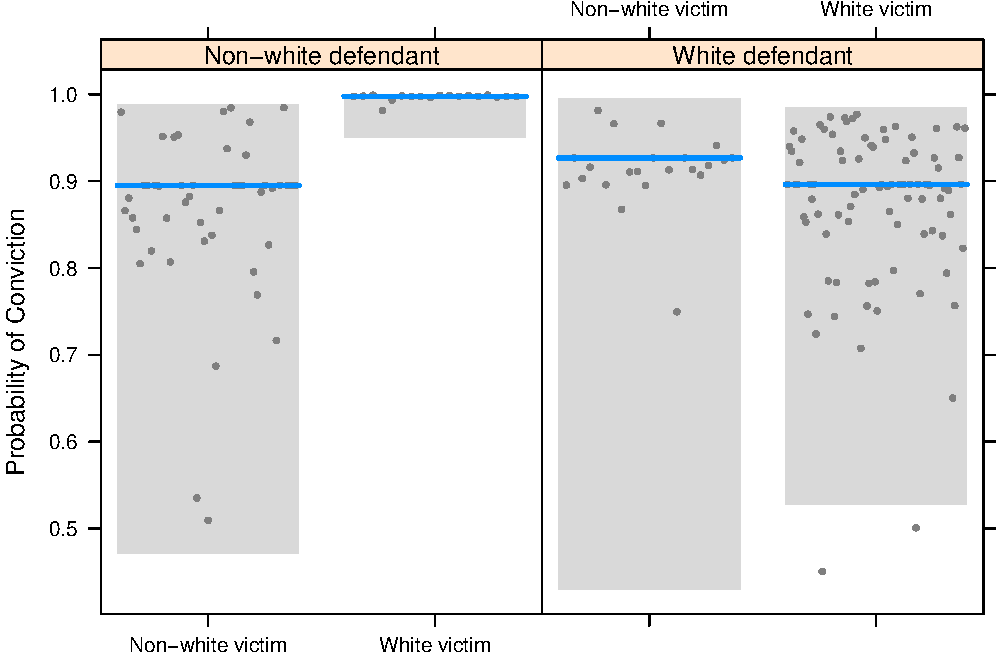
\includegraphics{stand_your_ground_article_files/figure-latex/unnamed-chunk-3.pdf}
\caption{Effect of Victim's Race on Probability of Conviction for White
and Non-White Defendants}
\end{figure}

\begin{figure}[htbp]
\centering
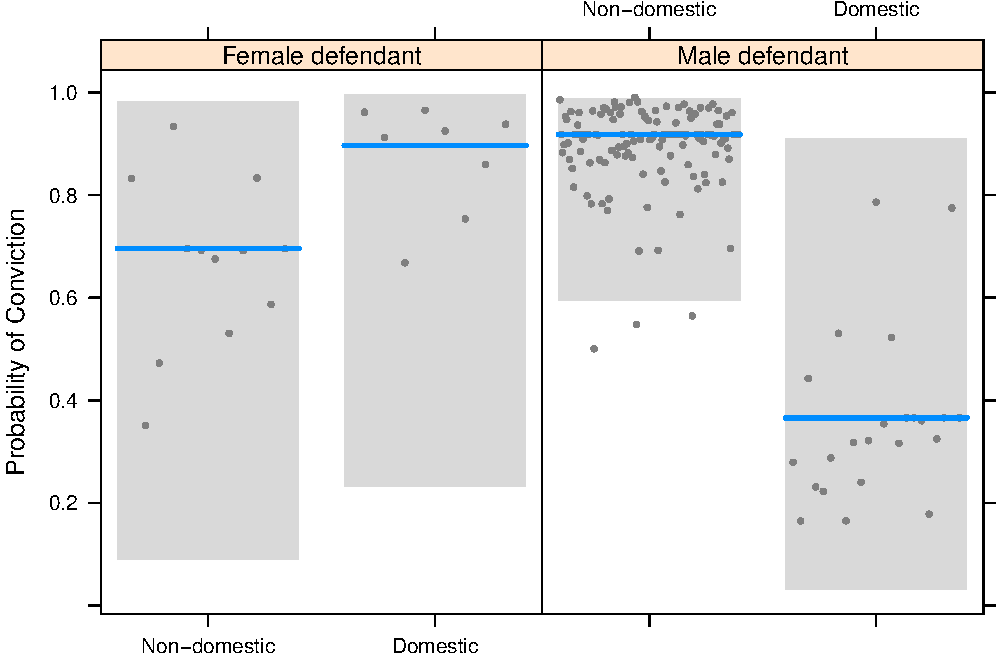
\includegraphics{stand_your_ground_article_files/figure-latex/unnamed-chunk-4.pdf}
\caption{lskjdflkj}
\end{figure}

\begin{figure}[htbp]
\centering
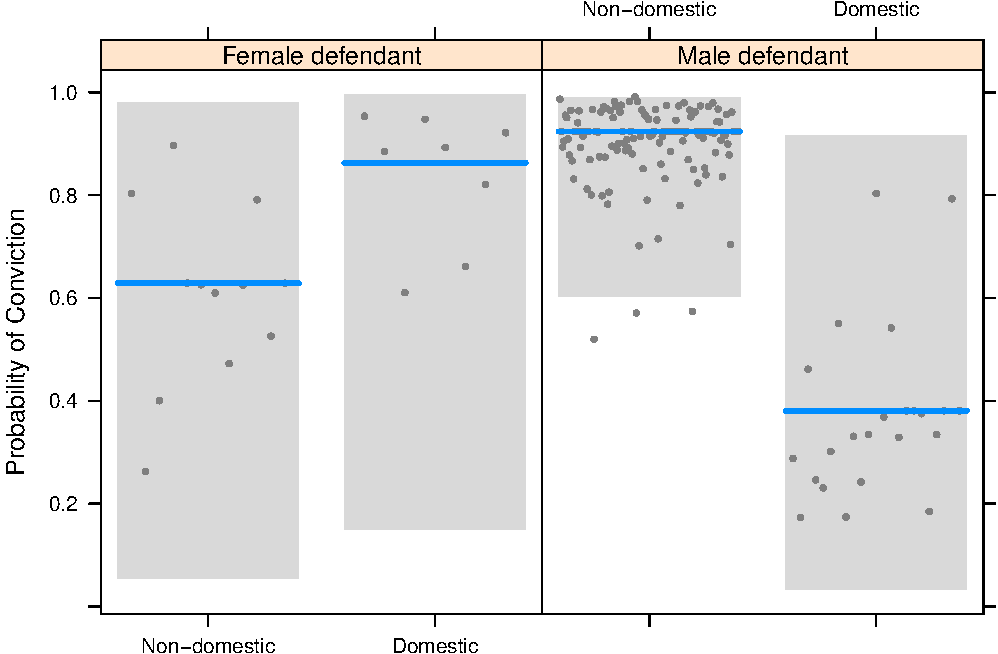
\includegraphics{stand_your_ground_article_files/figure-latex/unnamed-chunk-5.pdf}
\caption{lskjsdfsdfflkj}
\end{figure}

\subsection*{Conclusion}\label{conclusion}
\addcontentsline{toc}{subsection}{Conclusion}

Cheng, Cheng, and Mark Hoekstra. 2013. ``Does Strengthening Self-Defense
Law Deter Crime or Escalate Violence? Evidence from Expansions to Castle
Doctrine.'' \emph{Journal of Human Resources} 48 (3): 821--54.

John R Lott, Jr. 2013. ``Testimony Before the Senate.'' In \emph{Hearing
on "'Stand Your Ground' Laws: Civil Rights and Public Safety
Implications of the Expanded Use of Deadly Force}.

McCellan, Chandler, and Erdal Tekin. 2012. ``Stand Your Ground Laws,
Homicides, and Injuries.'' \emph{NBER Working Paper}, June.

Roman, John K. 2013. ``Race, Justifiable Homicide, and Stand Your Ground
Laws: Analysis of FBI Supplementary Homicide Report Data.''

\end{document}
